\subsection{C2 -- Solar lensing native window}\label{app:c2}
\paragraph{Native question.} Does the cited boundary/export window show the predicted shell qualification, push/pull split, torsional residual, and deflection/export witness?
\paragraph{Native readout.}
\begin{itemize}
\item cited window $\omega_{\mathrm{sol,lens}}$
\item structural key \texttt{tetron:4:4:8}
\item frame count / $T_{\mathrm{eval}}=512$ bip
\item weighting policy $w(\kappa)\equiv 1$
\item shell qualification
\end{itemize}
\paragraph{Native operator chain.}
\[
e_\alpha,\ e_\Omega,\ f
\;\to\;
q_{\mathrm{eff}},\ T_{\mathrm{tors}},\ \text{export witness}.
\]
\paragraph{Native output row.}
\begin{center}
\small
\begin{tabular}{lccccc}
\toprule
Row & Key & $q_{\mathrm{eff}}$ & $T_{\mathrm{tors}}$ & Export witness & Shell qualification \\
\midrule
C2.A & tetron:4:4:8 & $+1/2$ & 2 & emitted packet & qualified \\
\bottomrule
\end{tabular}
\end{center}
\paragraph{Temporal Conversion Block.} Temporal conversion is a normal chain-rule expansion on the cited native row. On this window, the lensing witness is
\[
1.7512432813682448\ \text{arcsec}.
\]
\paragraph{Native figure witness.}
\begin{center}
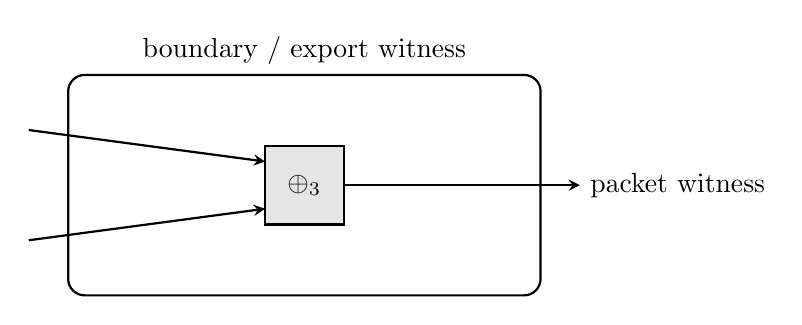
\begin{tikzpicture}[thick,>=stealth]
\draw[rounded corners=6pt] (0,0) rectangle (6,2.8);
\node[above] at (3,2.8) {boundary / export witness};
\draw[->] (-0.5,2.1) -- (2.5,1.7);
\draw[->] (-0.5,0.7) -- (2.5,1.1);
\draw[fill=gray!20] (2.5,0.9) rectangle (3.5,1.9);
\node at (3,1.4) {$\oplus_3$};
\draw[->] (3.5,1.4) -- (6.5,1.4);
\node[right] at (6.5,1.4) {packet witness};
\end{tikzpicture}
\end{center}
\paragraph{Hook / Evidence.} Use the cited shell/export and boundary-deflection hooks.
